\chapter{Experiment}

	This chapter will explore the ATLAS experiment in order to explain data specific to this analysis is obtained. First however is a discussion of the Large Hadron Collider which supplies the ATLAS experiment with proton collisions.

\section{The Large Hadron Collider}

	The Large Hadron Collider (LHC) is the largest and most powerful particle collider in the world with a circumference of $27~km$ and and design centre of mass collision energy of $14~TeV$. During the 2012 run the accelerator was run at a centre of mass energy of $8~TeV$ while providing an integrated luminosity of just above $20~fb^{-1}$ throughout the year to its two general purpose experiments, CMS and ATLAS, that latter of which provided data for this analysis.
	However the LHC can not run in isolation to provide beams for its 4 main experiments, instead it is the last and newest accelerator in a chain of accelerators which extract protons from a hydrogen canister with little to no momentum and inject them in to the LHC as a 450 GeV beam.
	The proton source is a device called a Duoplasmatron which injects hydrogen gas in to a strong electric field striping electrons from their nuclei. The remaining protons are injected in to Linac 2, a linear accelerator which accelerates them to an energy of $50~MeV$. The BOOSTER or Proton Synchrotron Booster (PBS) comes next in the chain and accelerates protons from $50~MeV$ to $1.4~GeV$ to be injected in to the main Proton Synchrotron (PS). The PS accelerates protons up to an energy of $25~GeV$ and again injects them in to another accelerator, the Super Proton Synchrotron (SPS). The SPS is the final stage before injection in to the LHC ring and pushes protons to an energy of $450~GeV$. Protons from the SPS then get injected in to the LHC in both counter revolving directions and accelerated to their final collision energy. For the data used in the analysis that follows (the 2012 data run) the final proton beam energy is $4~TeV$ giving a final centre of mass collision energy of $8~TeV$.

	The LHC itself is built in the same tunnel used by the Large Lepton-Positron (LEP) collider. Based at CERN (Centre of European Nuclear Research) the $27~km$ tunnel is between $50$ to $175~m$ underground and like CERN itself crosses the French-Swiss border just outside Geneva. Construction of the LHC started in 2001 after the LEP collider was decommissioned dismantled with excavation of the caverns for the LHC's four main experiments starting slightly before in 1998. 
	The LHC is a synchrotron machine requiring 1,232 super-conducting Niobium-Titanium dipole magnets each providing an $8.33~T$ magnetic field to direct the proton beams around its loop and an additional 392 quadrupole magnets of the same type to focus the beams for the collision points. The super conducting magnets operate at $1.9~K$ with the whole accelerator requiring 96 tonnes of liquid helium to remain cooled.\\

	-protons per bunch\\
	-number of bunches\\
	-luminosity (design and running for all of these)\\

	Four collision points exist around its circumference providing events to the four experiments; ATLAS (A Toroidal LHC Apparatus), CMS (Compact Muon Solenoid), ALICE (A Large Ion Collider Experiment) and LHCb (Large Hadron Collider beauty). ATLAS and CMS are both general purpose experiments designed to look for a variety of physics. ALICE is designed specifically to study quark-gluon plasma in heavy ion collisions scheduled for the end of each LHC run period while LHCb looks for beauty mesons in a search for CP-violation.
	There are also three additional LHC detectors in various stages of deployment without their own collision points; TOTEM (Total Elastic and diffractive cross section Measurement), LHCf (LHC forward) and MoEDAL (Monopole and Exotics Detector at the LHC) which measure separate beam properties. TOTEM shares CMS's collision point aiming to measure the proton cross-section very accurately while LHCf shares ATLAS's collision point measuring the very forward region of collision with the hope of investigating the source of ultra-high-energy cosmic rays. MoEDAL shares a cavern with LHCb and targeted to search for magnetic monopoles and other highly ionising stable massive particles.


\newpage

\section{ATLAS - A Toroidal LHC Apparatus}

	\begin{figure}[h]
		\begin{center}
			%\includegraphics[scale=0.1]{images/ATLAS_SE_Corrected7.eps}
		\end{center}
		\caption{Cut-away view of the ATLAS detector. The dimensions of the detector are 25 m in height and 44 m in length. The overall weight of the detector is approximately 7000 tonnes}
		\label{fig:ATLAS_cutaway}
	\end{figure}



	The ATLAS detector sits \SI{100}{\m} underground just over the road from the main CERN site and at \SI{45}{\m} long, \SI{25}{\m} in diameter and weighing over 7,000 tons is one of largest and most complex particle physics experiments in the world. The Detector it's self can be divided in to four main subsystems and from the interaction point out they are; the Inner Detector or tracking detector, the Calorimeters both Electro-Magnetic (EM) and Hadronic, the Magnet system and the Muon Spectrometer. There is also a small set of forward detectors, not detailed here, for accurate measurement of the integrated luminosity provided to ATLAS by the LHC named ALFA, LUCID and ZDC (reference?). 

	\begin{equation}
		\eta~=~-\ln[\tan(\frac{\theta}{2})]
	\end{equation}

	- detector coordinates system.\\
	- sub detector coverage and diagram.\\

	Broadly the detector is also divided in to the barrel region (cylinder surrounding the interaction point) and endcap region (circles covering the ends of the barrel region) which use slightly different configurations and technology in order to cover a full range in $\eta$.
	Following is a description of each main subsystem while focusing particularly on both the Inner Detector and EM Calorimeter as these are the important systems in identification of electrons used for this analysis.


	(- structured to hold it up?)

	\begin{tabular}{ | l | c | c | c | }
		\hline
		Detector component & Required resolution & \multicolumn{2}{|c|}{$\eta$ coverage} \\
		 & & Measurement & Trigger \\
    	\hline
    	\hline
    	Inner Detector & $\sigma_{p_{T}}/p_{T}~~=~0.05\%~p_{T}~\oplus~1\%$ & $|\eta|<2.5$ & N.A \\
    	\hline
    	EM calorimetry & $\sigma_{E}/E~=~10\%/\sqrt{E}~\oplus~0.7\%$ & $|\eta|<3.2$ & $|\eta|<2.5$ \\
    	\hline
    	Hadronic calorimetry (jets) &  &  &  \\
    	  barrel and end-cap & $\sigma_{E}/E~=~50\%/\sqrt{E}~\oplus~3\%$ & $|\eta|<3.2$ & $|\eta|<3.2$ \\
    	  forward  & $\sigma_{E}/E~=~100\%/\sqrt{E}~\oplus~10\%$ & $3.1<|\eta|<4.9$ & $3.1<|\eta|<4.9$ \\
    	\hline
    	Muon spectrometer & $\sigma_{p_{T}}/p_{T} =10\%$ at $p_{T} = 1$ TeV & $|\eta|<2.7$ & $|\eta|<2.4$ \\
    	\hline
    	%\caption{Table showing detector components resolution requirements and $\eta$ ranges when triggering and full measurement.}
    	\label{tab:det_res}
  	\end{tabular}

  	(- table of eta range, no. layers, output channels of every part of ID and CAL's)



	\subsection{Inner Detector}

		\begin{figure}[h]
			\begin{center}
				%\includegraphics[scale=0.175]{images/ID_newTRT_d3.eps}
			\end{center}
			\caption{Cut-away view of the ATLAS inner detector.}
			\label{fig:ATLAS_inner}
		\end{figure}

		The Inner Detector is ATLAS's main tracking detector fitted as the closest part to the interaction point. A tracking detector is needed to trace charged particles from the interaction point out to the calorimetry system and give two bits of information; a charged particles position to match with the calorimeters (or Muon Spectrometer in the case of muons) and when a magnetic field is present an estimate of a particles momentum to compare with the calorimeter obtained from the radius of its curve. It is composed of three different tracking technologies in order going out from the collision point; the Pixel Detector (PD), the Semiconductor Tracker (SCT) and the Transition Radiation Tracker (TRT). The Inner Detector was designed to precisely measure charged tracks in the energy range 0.5 GeV - 150 GeV while complimenting the energy measurements of the Calorimetry system. Covering a range of $|\eta|~<~2.5$ and full range in $\phi$ the Inner Detector with the help of the 2 T magnetic field imposed by the solenoid magnet (discussed bellow) boasts a momentum resolution of $\sigma_{p_{T}}/p_{T}~=~0.05\%~p_{T}~\oplus~1\%$ to charged tracks. In its design it was also important for the Inner Detector to be able to distinguish between multiple primary vertices at the collision point, referred to as pile-up, as well as secondary vertices from sources such as the hadronisation of b quarks. 
		(-stats as to precision?)

		\begin{figure}[h]
			\begin{center}
				%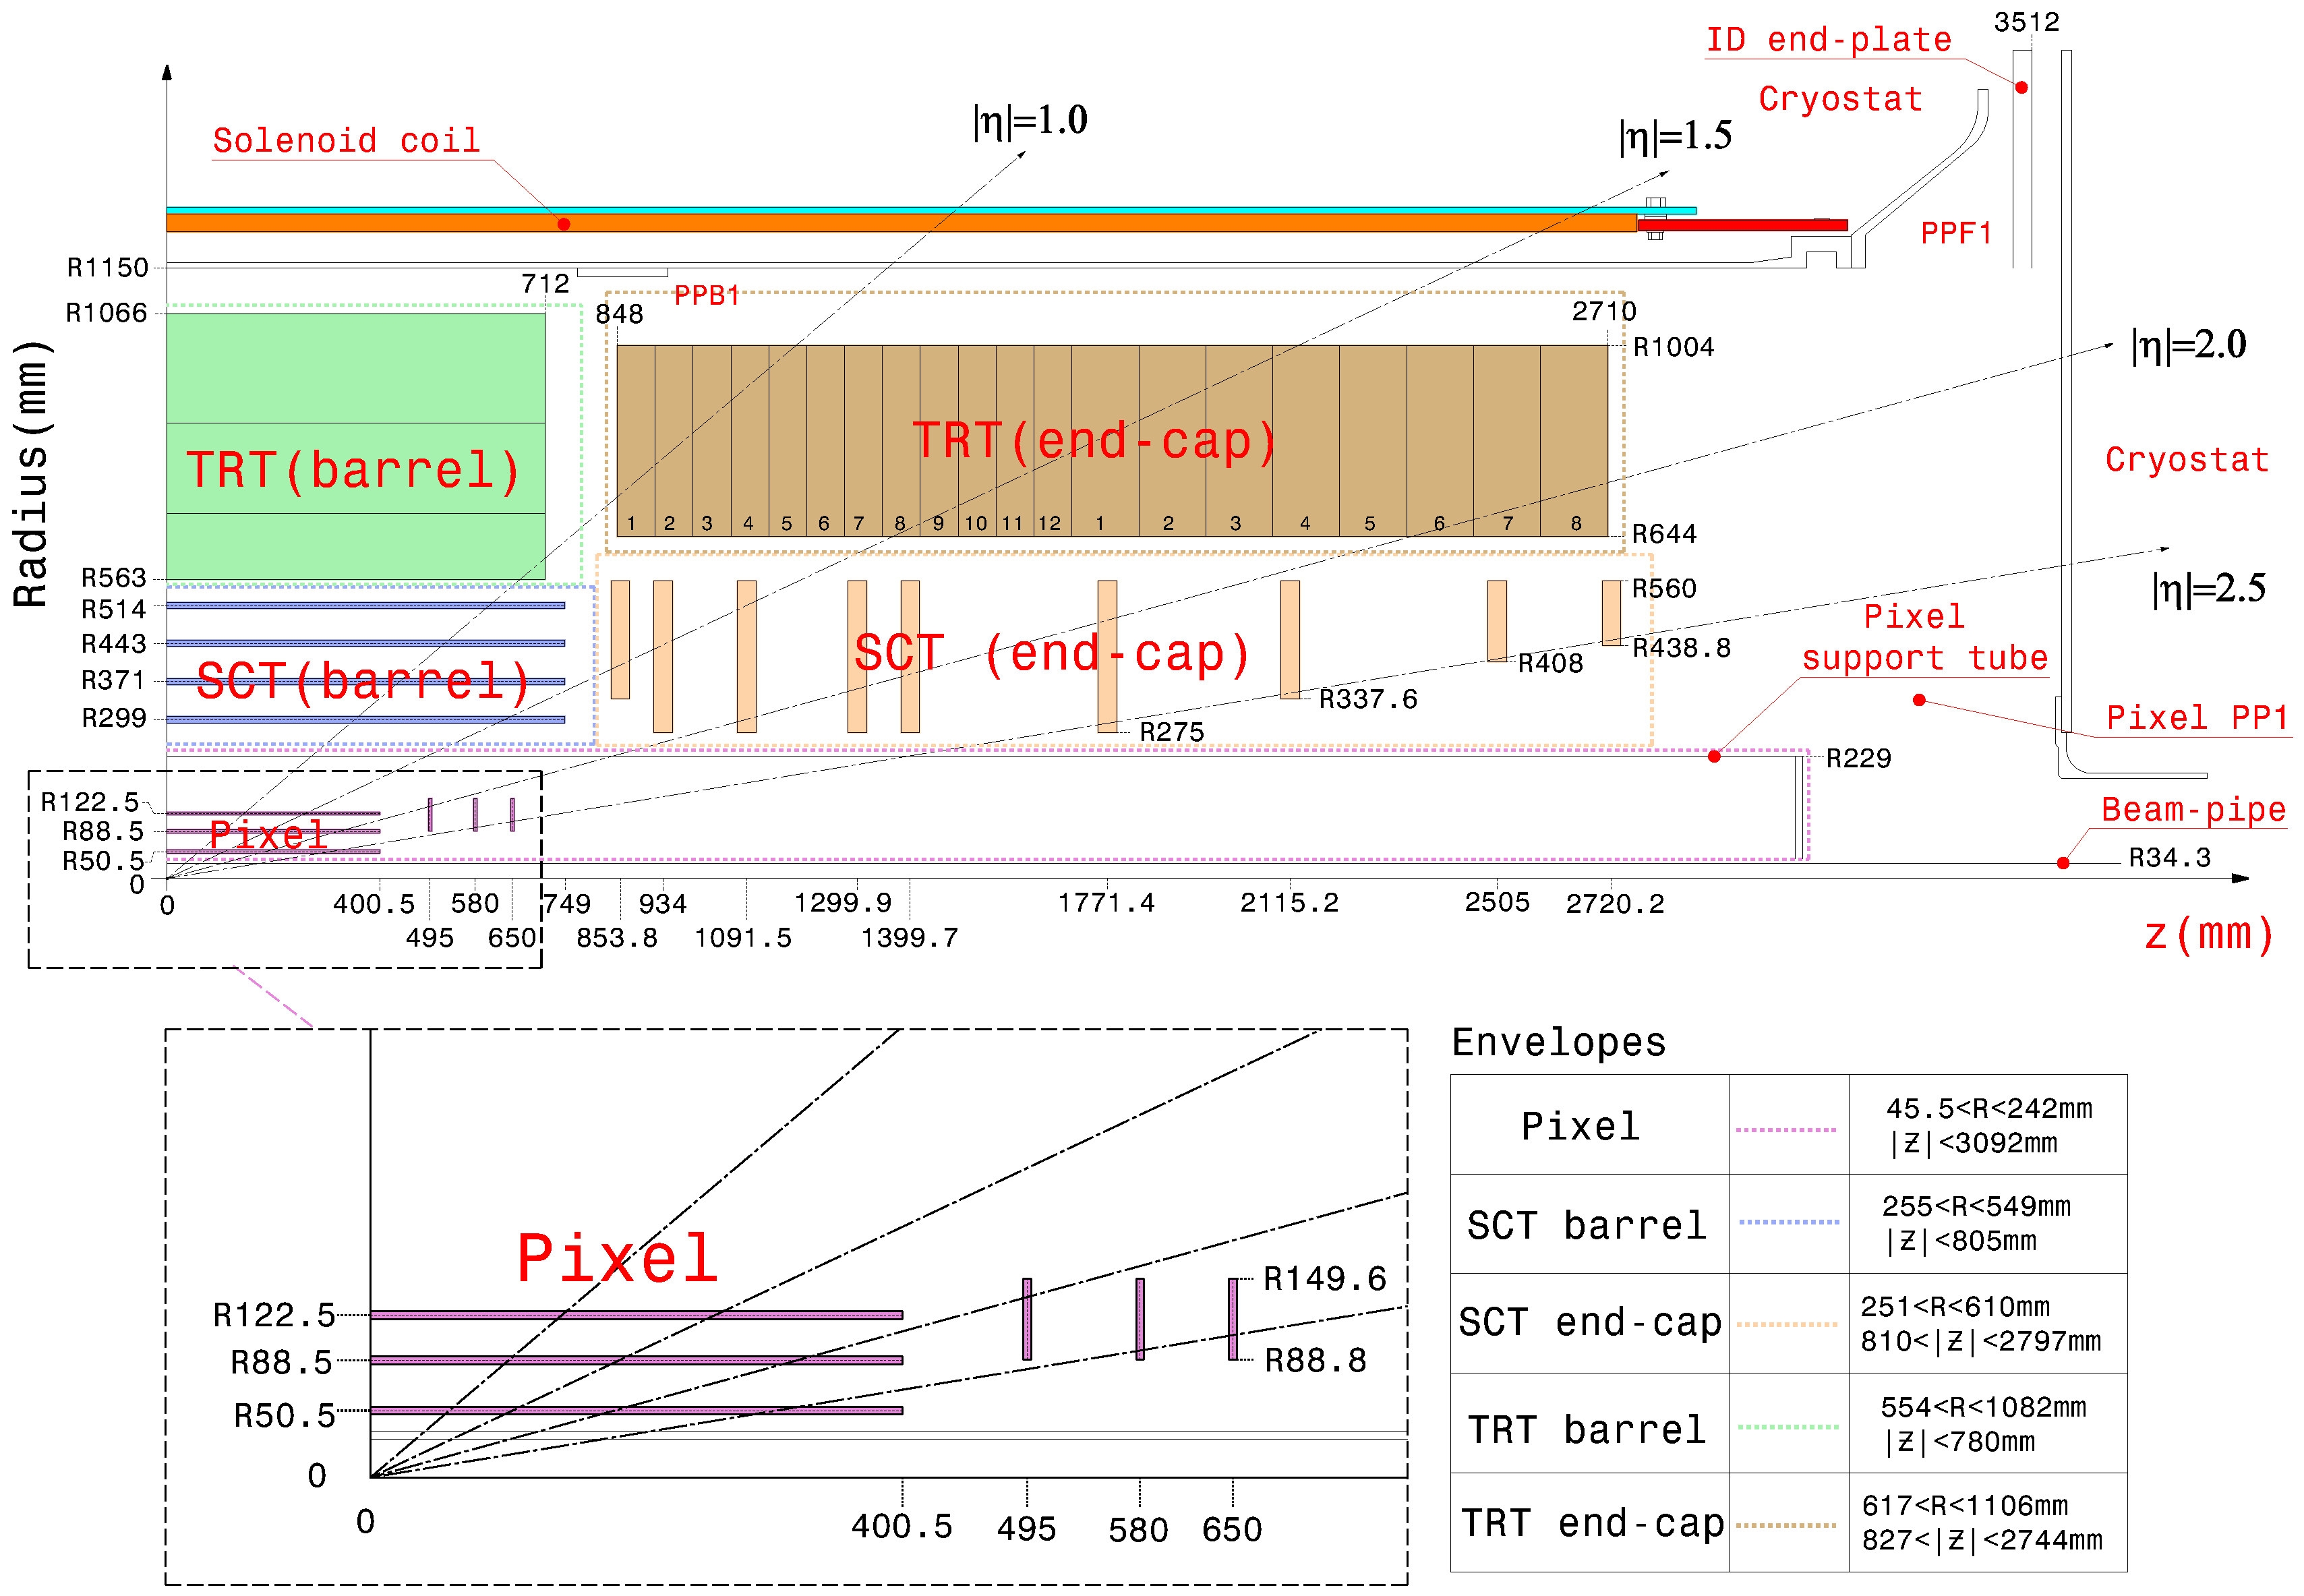
\includegraphics[scale=0.3]{images/FigID26-mod-011107.eps}
			\end{center}
			\caption{Plan view of a quarter-section of the ATLAS inner detector showing each of the major
detector elements with its active dimensions and envelopes.}
			\label{fig:ATLAS_inner_config}
		\end{figure}



		\subsubsection*{Pixel Detector} 

		The Pixel Detector is the first layer and closest to the beam line consisting of three layers of silicon pixels. Because of its proximity to the beam line the pixel detector are designed to be heavily radiation hard and understood to the degree that its performance can be predicted over an extended period of radiation exposure. The Pixel Detector is made of a barrel and two endcaps composed of 1744 modules all together. \\
		(- each module, no. pixels)
		(- keep cool to avoid leakage current.)
		(-read out channels?)


		\subsubsection*{Semiconductor Tracker}

		The SCT consists of the same technology as the PD but organised in to four layers in the barrel region and 9 layers in each endcap. Due to the amount of electronics cooling is rather important to this layer and so the sensors in each module are glued to each side of a thermally conductive spine that gives the SCT structure and transports heat out via the mounting point of each module keeping them at their operating temperature of \SI{-7}{\degreeCelsius}.\\
		(-read out channels?)



		\subsubsection*{Transition Radiation Tracker}

		The TRT uses a completely different tracking technology to the rest of Inner detector it uses a straw detectors composed of 4 mm diameter polymide tubes each with a \SI{31}{\um} diameter gold plated Tungsten-Rhenium wire. Due to the small diameter of straws the TRT can obtain the high read-out rate needed for experiments at the LHC. The barrel region consists of 50,000 of these straws with a readout at each end providing 100,000 readout channels. The endcaps contain another 320,000 straws only read out a one end giving the TRT a total of 420,000 channels. Each channel measures drift time giving a resolution of \SI{170}{\um} in each straw. The straws are filled with a high Xenon concentration (\ce{Xe}(70\%)\ce{CO2}(27\%)\ce{O2}(3\%)) of gas in order to detect electrons via radiated photons as they traverse the material between straws (-what is this material?). This is achieved by giving each straw two timing thresholds, the lower to discriminate tracking hits (direct hits) while the higher threshold discriminates transition radiation hits. \\
		(-eta ranges of barrel end cap.)
		(-number of straw hits in each region) 
		



	\subsection{Calorimeters}

		\begin{figure}[h]
			\begin{center}
				%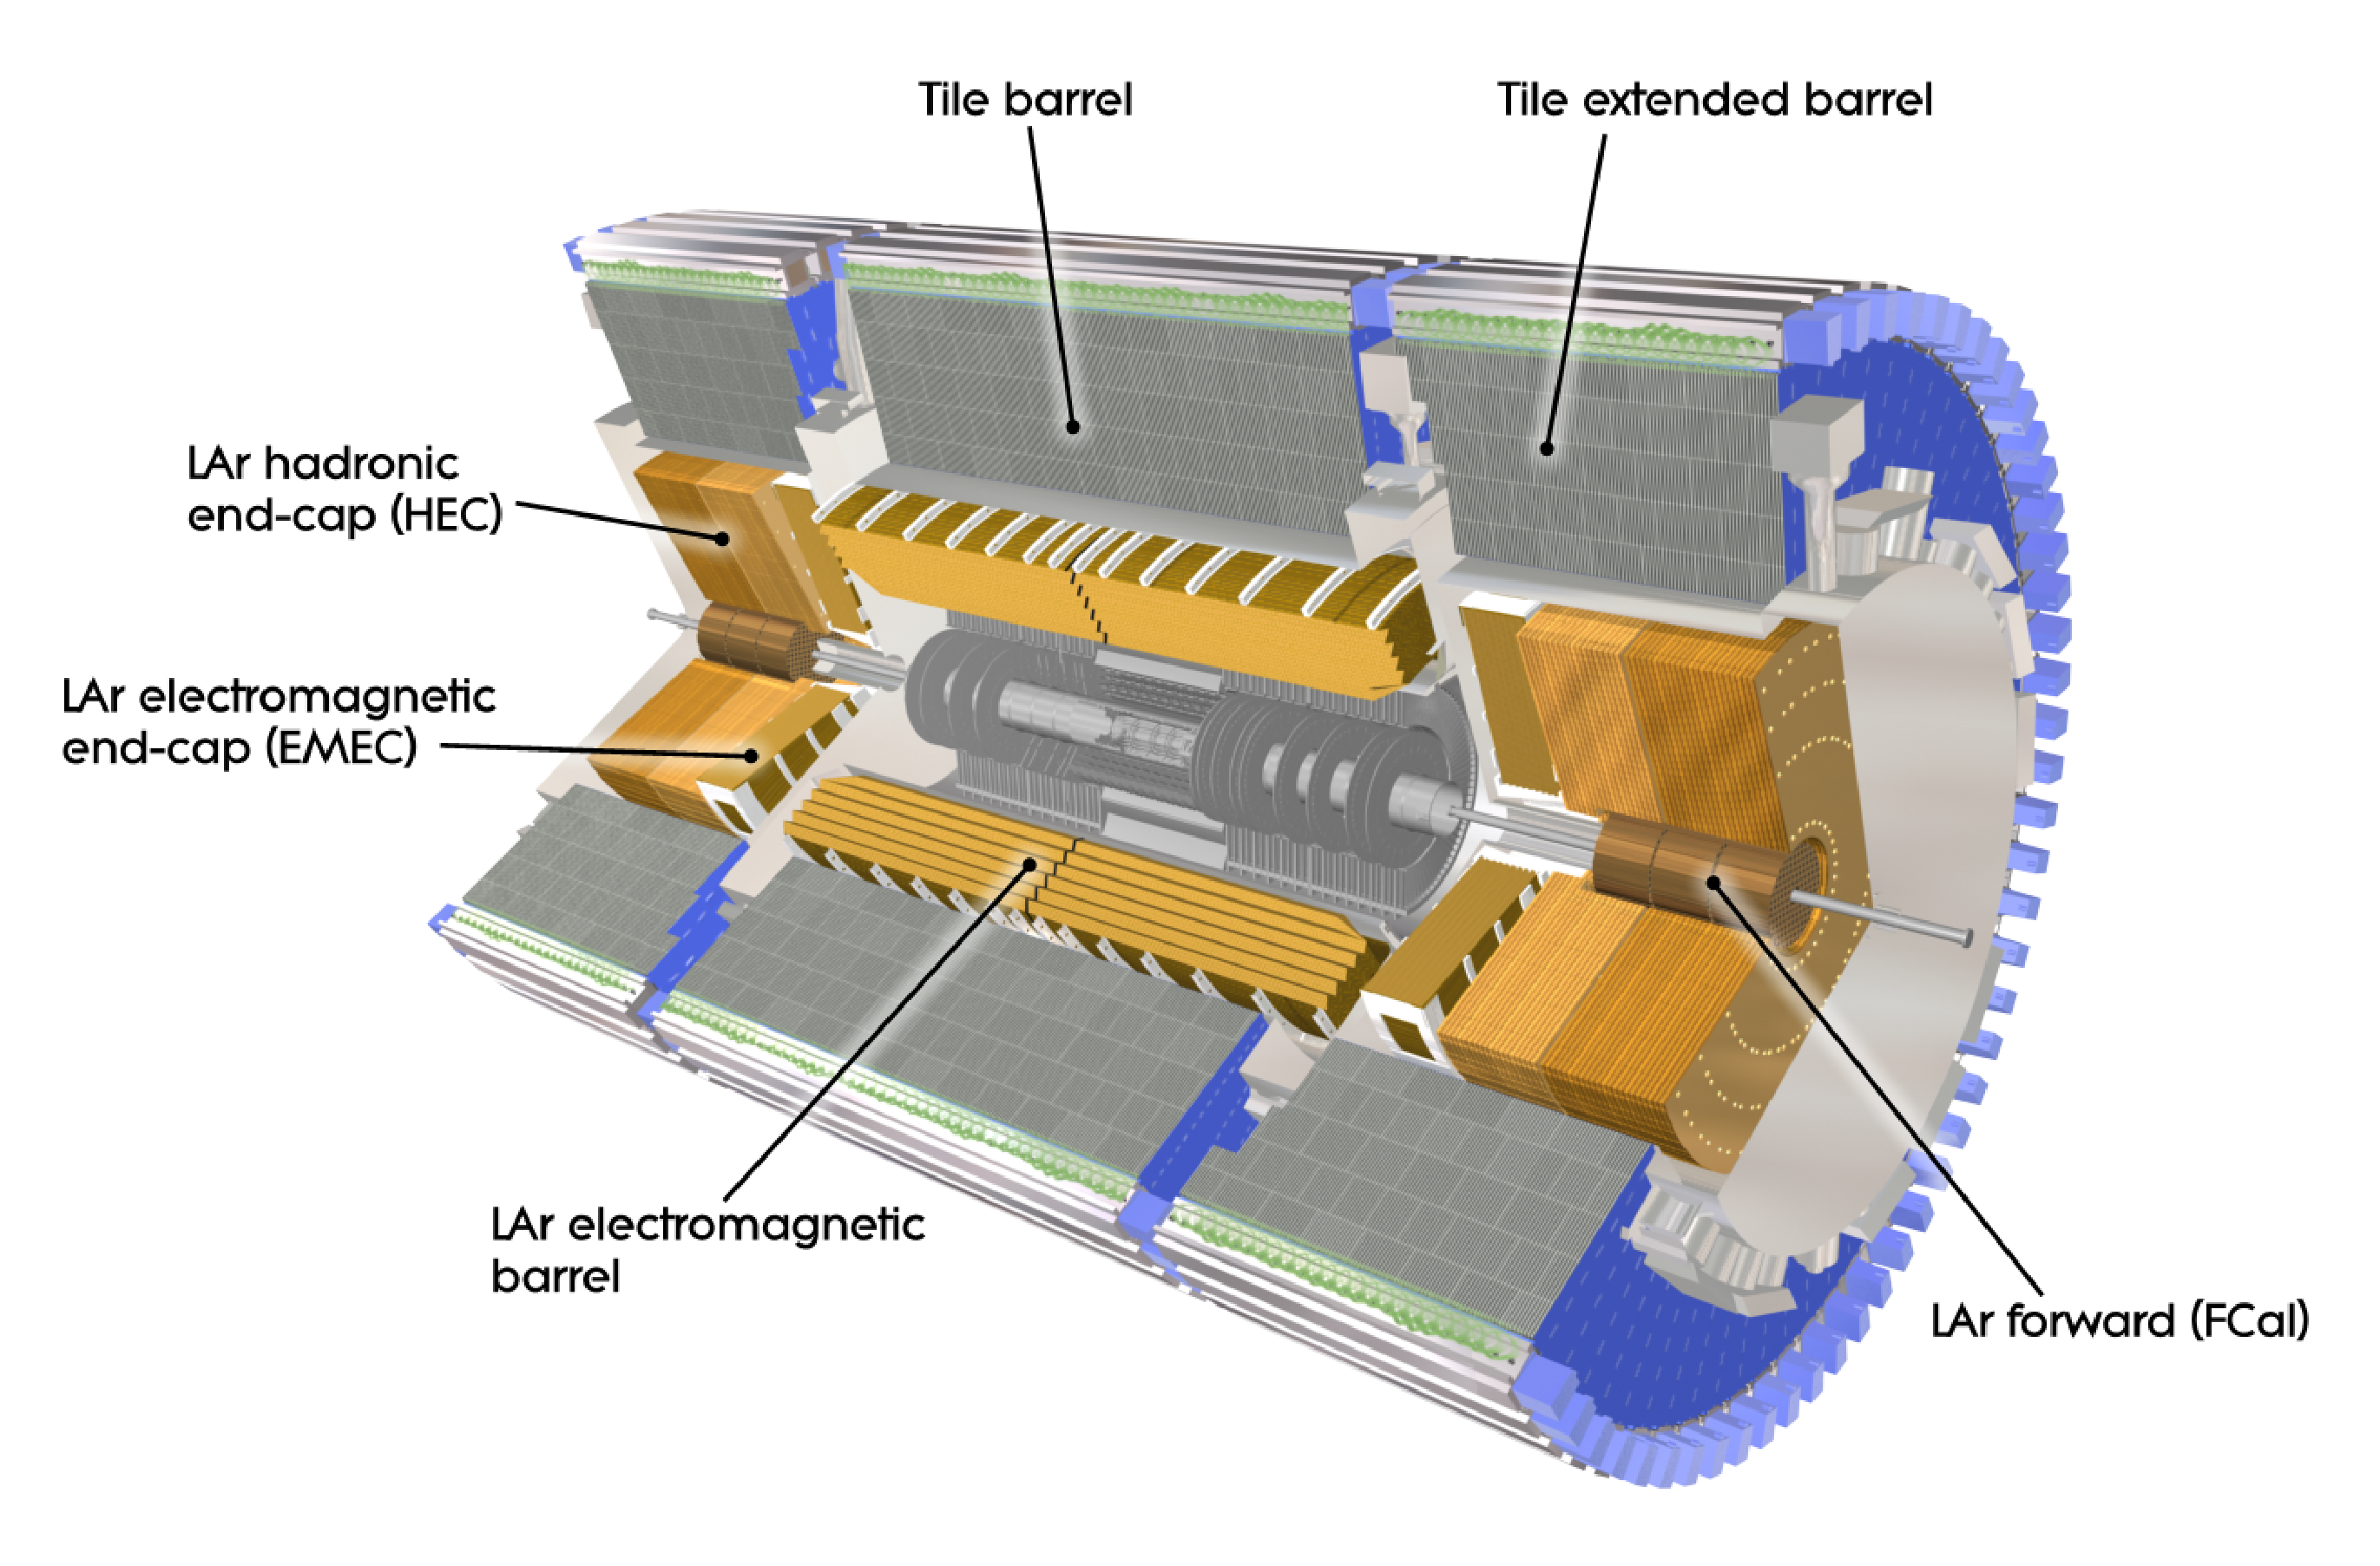
\includegraphics[scale=0.35]{images/Calorimeter_d3.eps}
			\end{center}
			\caption{Cut-away view of the ATLAS calorimeter system.}
			\label{fig:ATLAS_calo}
		\end{figure}

		While the Inner Detector only measures charged particles, the Calorimeters measure both neutral and charged particles and is split in to two different for particles with differing properties. The inner Electromagnetic Calorimeter is designed primarily to measure electrons and photons as well as pions while the outer Hadronic Calorimeter looks for hadrons such as neutrons and protons although in analyses the Hadronic calorimeter is primarily used to look for jet objects (a collection of particles issuing from the decay of one mother particle). The primary method of identifying charged particles is to look for an associated track in the inner detector although the shape of the energy deposit in the calorimeters also helps with identification.

		(- radiation thickness of detector)
		(- prevent leakage in to next layer)


		\begin{figure}[h]
			\begin{center}
				%\includegraphics[scale=0.5]{images/ITCconcept_new.eps}
			\end{center}
			\caption{Schematic of the transition region between the barrel and end-cap cryostat's.}
			\label{fig:ATLAS_calo_crack}
		\end{figure}


		\subsubsection*{Electromagnetic Calorimeter}

		The Electromagnetic Calorimeter (ECAL) is designed to fully stop all electromagnetic showers within its volume. Split in to a barrel section and two endcaps the ECAL uses Liquid Argon (LAr) as a detecting medium with lead as the absorber. The lead is arranged in an accordion fashion (seen in *) to ensure consistent performance throughout $\phi$. In the barrel section a presampler of LAr type is found before the main calorimeter to correct later sub-detectors for dead material. The barrel contains three layers of LAr modules of decreasing size in towards the collision point in order to keep good position resolution. The endcap only contains two layers of modules while with a similar ideal.\\

		(- shape information and electons/photons/pions)
		(- energy resolution)
		(- forward calorimeters)

		\subsubsection*{Hadronic Calorimeter}

		The Hadronic calorimeter is designed to stop all hadronic showers within its volume and consists of two parts, the Tile Calorimeter (HCAL) in the barrel and the LAr Hadronic Endcap (HEC). The HCAL is a title calorimeter consisting of alternating layers of scintillator and steel and the active medium and absorber respectively. The HEC on the other hand uses the same technology as the ECAL copper plates and filled with LAr as the detecting medium. As the Hadronic calorimeter sits directly behind the ECAL it is useful in the detection of electrons as a measurement of hadronic isolation can be found or the amount of leakage in to the HCAL from a electron shower in the ECAL.\\
		(- eta ranges?)
		(- forward calorimeters)
		


	\subsection{Magnet System}

		
		\begin{figure}[h]
			\begin{center}
				%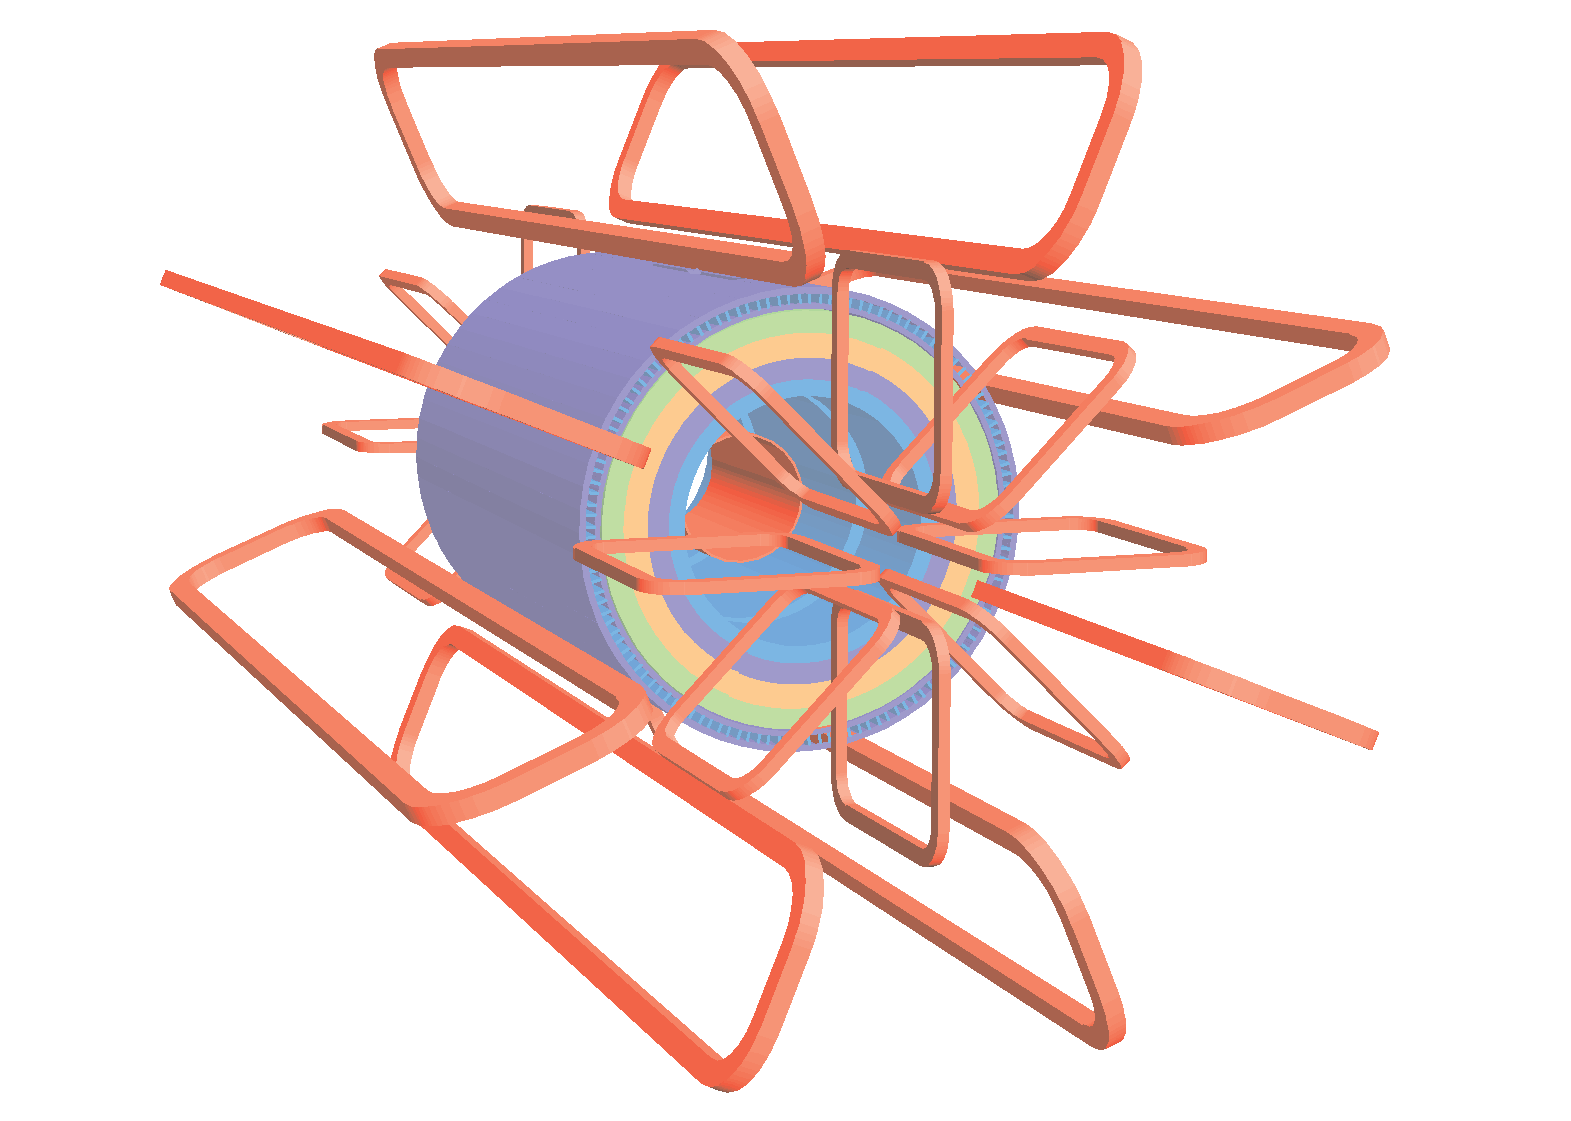
\includegraphics[scale=0.3]{images/ATLcoilGeom.eps}
				%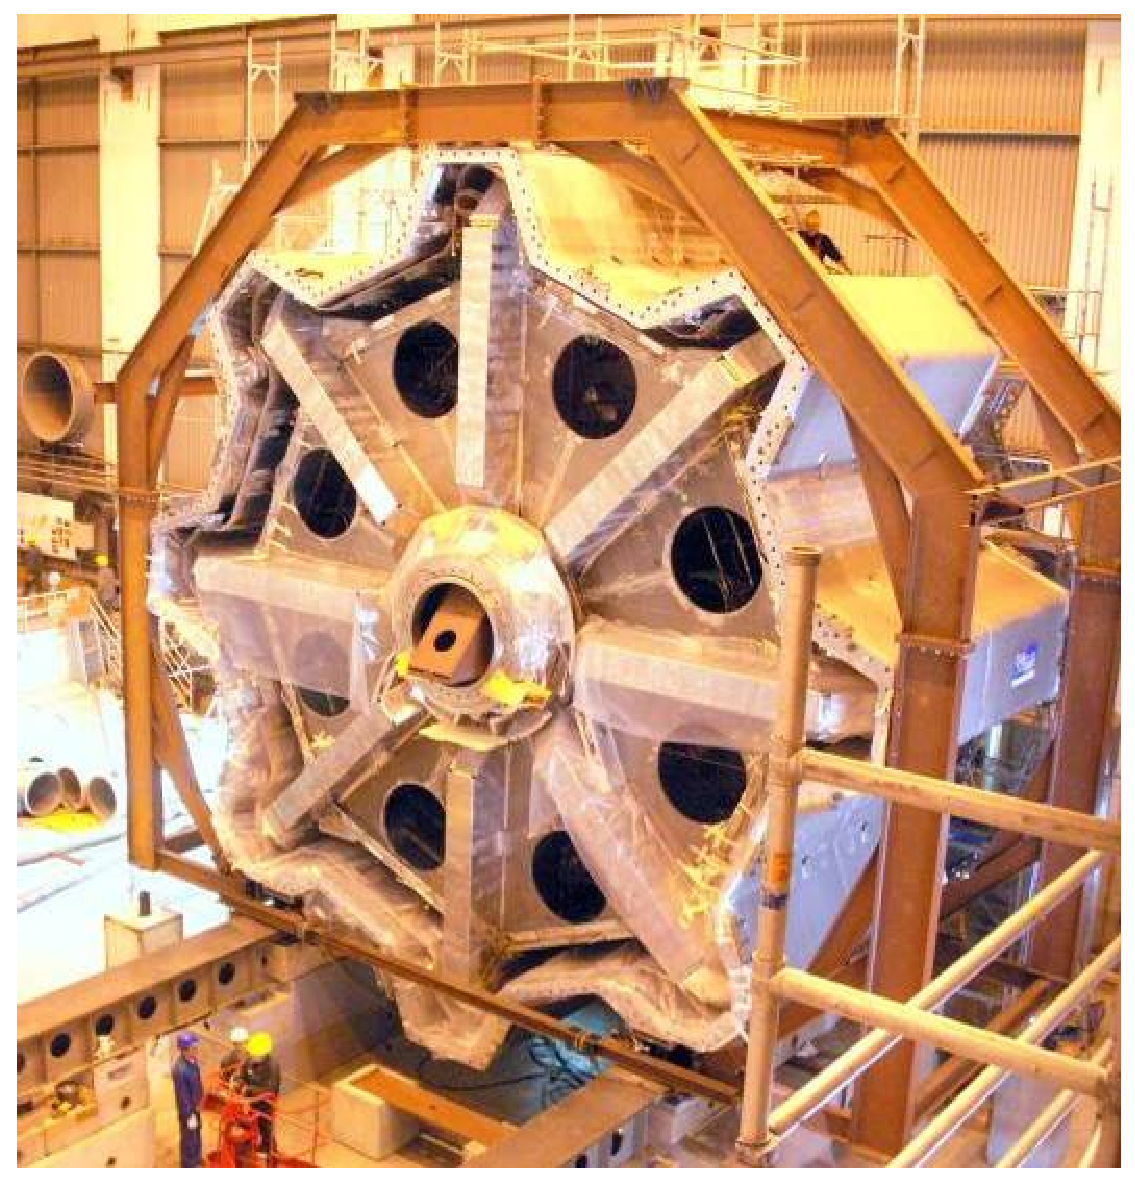
\includegraphics[scale=0.3]{images/desc5.eps}\\
				%\includegraphics[scale=0.3]{images/desc6.eps}
			\end{center}
			\caption{Geometry of magnet windings and tile calorimeter steel, end-cap toroid cold mass inserted into the cryostat and barrel toroid as installed in the underground cavern.}
			\label{fig:ATLAS_magnet}
		\end{figure}

		The ATLAS detector has two main magnet systems, the inner solenoid magnet found between the TRT and the ECAL and the outer toroid magnets found interleaved with the Muon Spectrometer. 

		The solenoid system is a super conducting magnet is kept at \SI{4.6}{\K} (check?) to provide the \SI{2}{T} magnetic field required by the inner detector to curve high energy particles found at the LHC. As the solenoid is found inside the calorimetry system it is important radiative thickness is minimised to reduce efficiency losses in energy measurements. In order to achieve this it was designed to minimise dead material and shares its cryostat vessel with the ECAL reducing the need for two and therefore contributing only 0.63 radiation lengths.\\ 
		(-materials)

		The outer toroid system provides a magnetic field for the muon spectrometer and consists of a barrel and two endcap systems each with eight coils assembled radially around the beam axis. The coils are all aluminium stabilised Niobium-Titanium (\ce{NbTi}) superconductors with each coil in the barrel contained in its own cryostat while each of the coils in the endcap systems are contained in one single cryostat each. The peak field provided by these toroids are \SI{3.9}{T} and \SI{4.1}{T} in the barrel and endcap's respectively.\\
		(-temp?)

	


	\subsection{Muon Spectrometer}

		\begin{figure}[h]
			\begin{center}
				%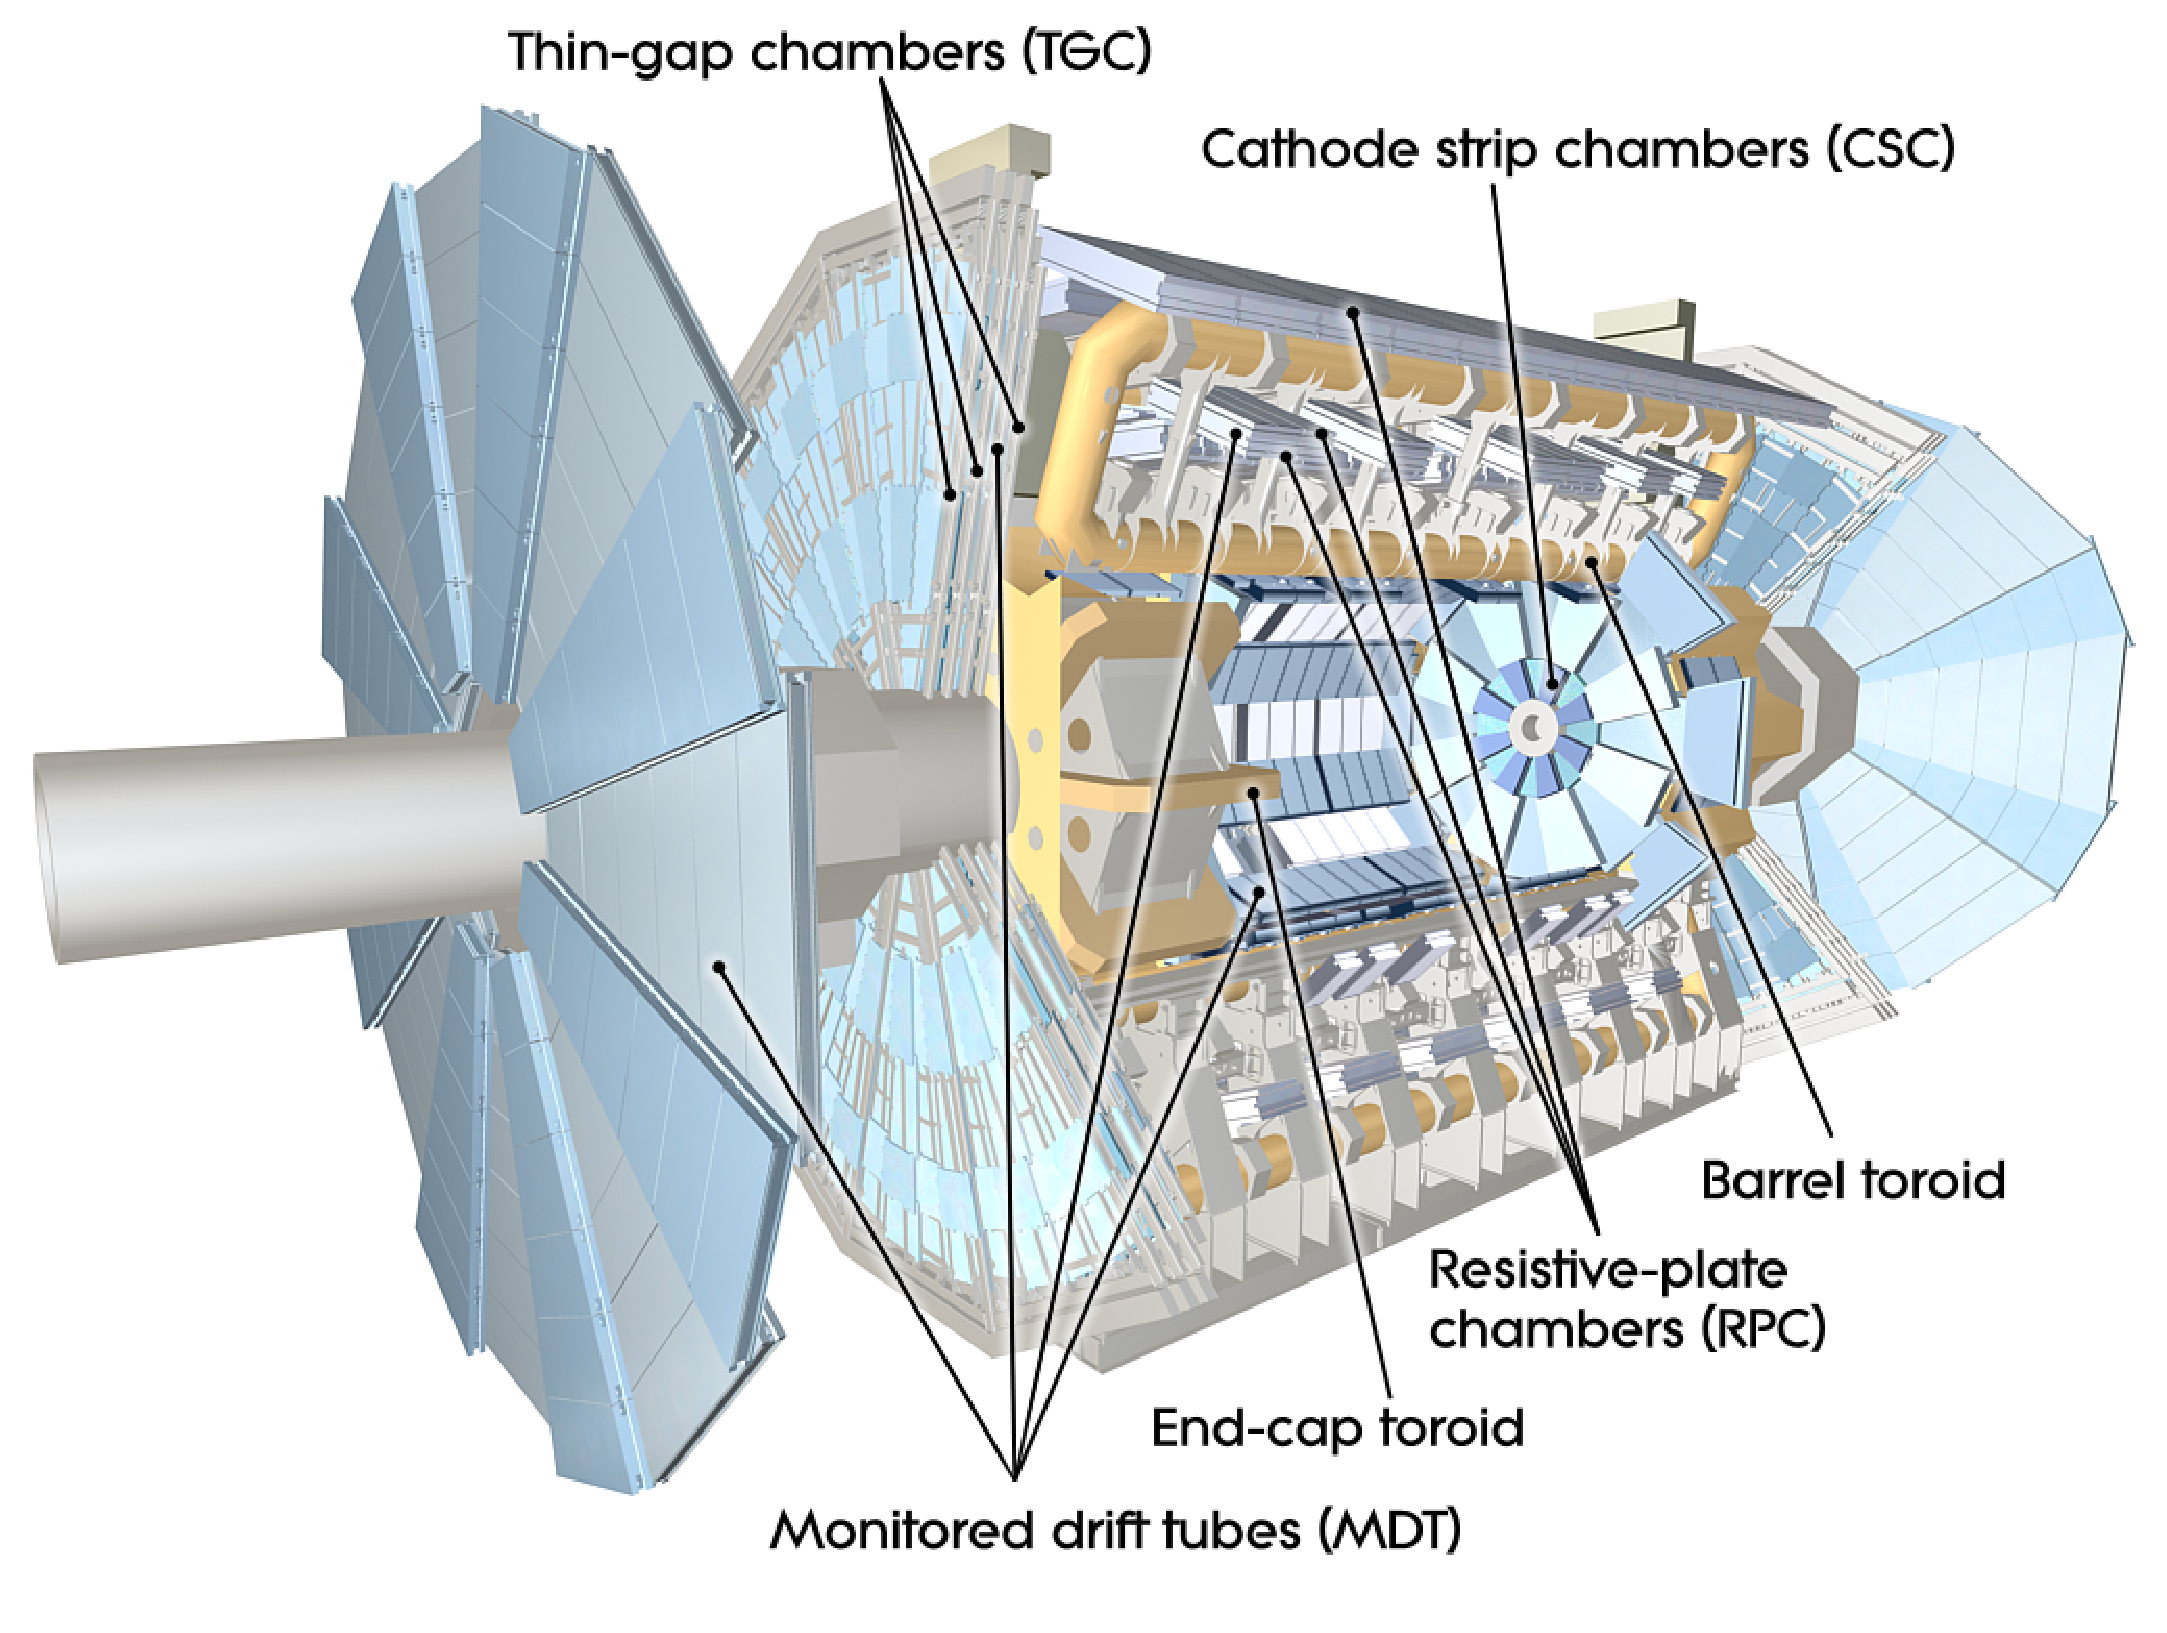
\includegraphics[scale=0.4]{images/MuonSystem_d3.eps}
			\end{center}
			\caption{ Cut-away view of the ATLAS muon system.}
			\label{fig:ATLAS_muon}
		\end{figure}

		Due the penetrative nature of muons all the layers of detector discussed above do not induce the showering of high energy muons. Therefore the outermost detector is another tracking detector specifically for muons and uses the outer toroid magnet system to measure muon momentum. The Muon Spectrometer is composed to 4 different technologies; Monitor Drift Tubes (MDT), Cathode Strip Chambers (CSC), Resistive Plate Chambers (RPC) and Thin Gap Chambers (TGC). Both the MDT and the CSC boast precision tracking though both have slow readout times. This leaves the RPC and TGC the job of triggering muons and providing additional track measurements. The RPC are found in the barrel region ($|\eta|~<~1.05$) while the TGC trigger in the endcap region ($1.05~<~|\eta|~<~2.4$) and the MDT covers a full range in $\eta$ ($|\eta|~<~2.7$) with complementary measurements from the CSC at $2.0~<~|\eta|~<~2.7$.\\
		(- detector alignment)
		(- no. chambers?)



%\section{The Tracking Detector and Electrons}


%\section{The Calorimeters and Electrons}
